%==============================================================================
% Template research proposal bachelor thesis
%==============================================================================

\documentclass[english]{hogent-article}

% Specify bibliography file
\addbibresource{references.bib}

% Information about the study programme, course, assignment
\studyprogramme{Professional bachelor applied computer science}
\course{Research Methods}
\assignmenttype{Paper Research Methods: research proposal}
\academicyear{2024-2025}

\title{Object Recognition and Data Visualization of Observations with Tobii Eyetracking Glasses in Healthcare Simulations.}

\author{Ilian Bronchart}
\email{ilian.bronchart@student.hogent.be}

% TODO (phase 1): Give the link to your Github-repository here
\projectrepo{https://github.com/HoGentTIN/paper-research-methods-en-24-25-rmilian}

\specialisation{AI \& Data Engineering}
% Enter some keywords here that describe your topic
\keywords{Object Detection, Eyetracking, Healthcare Simulations, Pedagogy, Nursing}

\begin{document}

\begin{abstract}
Observational skills of healthcare professionals are a cornerstone of accurate diagnoses and empathic patient support. 
To cultivate these skills, healthcare education increasingly employs simulated environments, 
like HOGENT's 360° Care-lab, where students learn to interact with patients and identify visual cues. 
Currently, the evaluation of these skills often relies on traditional methods such as student 
self-reporting and direct instructor observation, which are inherently subjective, and may not 
consistently capture the nuances of student performance. 
While the Care-lab's Tobii eyetracking glasses provide objective gaze data, a key limitation is the absence 
of dedicated software to automatically analyze what students observe and for how long.
This research aims to address this deficiency by integrating computer vision models with eyetracking data, 
thereby enabling automated analysis and visualization of student observational performance to enhance trainer feedback.

The core of the methodology is the development of a proof-of-concept (PoC) software solution. 
This process starts with a literature review of eyetracking analysis and relevant computer vision techniques, 
and proceeds to the design and implementation of a prototype application, featuring a data-labeling tool. 
Further steps involve conducting controlled experiments in HOGENT's 360° Care-lab, 
where students using Tobii Pro Glasses 3 will generate eyetracking recordings during simulated tasks. 
These recordings will be labeled using the aforementioned tool to establish a ground-truth dataset, 
against which various computer vision models will be integrated and evaluated for their 
performance.

It is expected that the PoC software will successfully demonstrate the automated identification 
of objects viewed by students and the precise measurement of their gaze duration. 
Ultimately, this research aims to provide trainers with an objective, data-driven tool to more effectively assess 
student observational skills, thereby enhancing feedback mechanisms and improving the overall efficacy of healthcare simulation training.
\end{abstract}

\tableofcontents

\bigskip

\paragraph{Remark}

I'm also working on the bachelor's thesis this year. The content of this research proposal also serves as the subject for my bachelor thesis. 
My promoter is Mr. Bert Van Vreckem. The scope and objectives presented here represent an evolution from the initial proposal submitted 
for the bachelor's thesis, reflecting a deeper understanding gained through preliminary research and development.

The original proposal focused broadly on integrating object detection and segmentation with Tobii Glasses data for automated analysis and visualization.
Upon reflection, and while the core research question remains consistent, this\\ improved proposal refines the 
methodology and deliverables into a more structured approach. 
The initial research sub-questions were\\ predominantly oriented towards the solution domain, exploring specific models and\\ technical methods.
Here, a better balance is\\ achieved by first incorporating sub-questions\\ that apply to the problem domain, such as understanding current barriers and user needs, before addressing solution-specific inquiries.
Furthermore, where the initial proposal outlined a general user flow for the PoC, 
this proposal articulates the overall goal through distinct, actionable sub-objectives.
This offers a clearer roadmap with more defined milestones.
Additionally, this proposal places emphasis on the development of the labeling tool and the subsequent creation of a ground-truth dataset as foundational steps.
This aspect, while important for any credible evaluation of automated analysis methods, was less prominent in the original submission.

It is acknowledged that the scope of this research is ambitious, particularly concerning the development of a 
prototype labeling application, experimental work, and the implementation and evaluation of multiple computer vision models.
This ambition is supported by a dedicated work schedule: having completed my internship in the first semester, the second semester allows for a more intensive focus
on the bachelor's thesis, with significantly more dedicated time per week than is typical for students undertaking their thesis concurrently with their internship.
Moreover, this ambitious scope also serves as an opportunity to demonstrate a well-rounded skillset as a software engineer, showcasing expertise in front-end development, back-end development, and data science.

\section{Introduction}
\label{sec:Introduction}

The observational skills of healthcare providers are fundamental, not only for achieving\\ accurate diagnoses but also for effectively supporting and guiding patients through their care.
In contemporary healthcare education,\\ simulation-based training plays a pivotal role in preparing students for real-world scenarios.
At HOGENT, the 360° Care-lab offers an environment where students engage in realistic scenarios,\\ such as a simulated hospital room with a mannequin patient, or a patient's living room.
Here, students practice interacting with patients and learn to identify important visual cues in their environment.
Examples range from recognizing a soft drink bottle on the nightstand of a patient with diabetes, to observing a picture frame on the wall that may serve as a conversation starter.
This training aims to connect a student's theoretical knowledge with practical skills, thereby preparing them for the complexities of real-world healthcare settings.

Despite the advancements in\\ simulation-based training, the evaluation of students' observational skills often relies on traditional methods such as student self-reporting\\ and direct observation by instructors.\\
These methods are inherently subjective and may not reliably capture the full spectrum of a student's performance.
To address this, the Care-lab is equipped with Tobii eyetracking glasses, which can objectively record students' eye movements and their field of view. 
While the technology offers a wealth of data, previous efforts at the Care-lab focused primarily on analyzing gaze paths.
This approach, however, still required trainers to manually review each recording and did not produce objective metrics to quantify student performance efficiently.
This highlights a significant challenge for the instructors at the Care-lab, who require more effective tools to provide feedback to students.

The problem statement guiding this research is as follows: Although the Tobii eyetracking\\ glasses provide valuable objective data, there is currently no suitable software to automatically analyze whether
students have indeed observed the relevant objects within the simulation. This deficiency in automated data processing makes the assessment of students' observational skills both time-consuming and subjective.

This leads to the central research question of this study:
\textit{How can computer vision models be integrated with eyetracking data from\\ Tobii Glasses to automatically analyze and visualize the observational performance of students in HOGENT's 360° Care-lab?}
This overarching question will be explored through several sub-questions:
\begin{itemize}
  \item What are the barriers experienced with current manual observation methods?
  \item What are the user needs for interpreting and analyzing eyetracking data in the\\ current context?
  \item Which features should an automated analysis method have to address the limitations of manual observation?
  \item To what extent can the models and developed software:
    \begin{enumerate}
      \item accurately determine which critical objects students have observed?
      \item precisely measure how long\\ students have looked at these objects?
    \end{enumerate}
\end{itemize}

The primary objective is to develop and evaluate a proof-of-concept (PoC) software system designed to automate the analysis of students' observational performance in the Care-lab.
This system will integrate eyetracking data from the Tobii Pro Glasses 3 with computer vision models to identify observed critical objects and quantify the duration of gaze upon them.
The pursuit of this objective will be structured through the following key deliverables and activities, to be completed within the timeframe of this research:
\begin{enumerate}
    \item \textbf{Development of a prototype labeling application:} A functional software tool will be created, featuring a user-friendly interface.
    This application will enable trainers at the Care-lab to efficiently annotate objects\\ within the various simulation environments.
    The output of this application will be a labeled dataset, which will serve as the foundation for training and evaluating computer vision models.
    \item \textbf{Experimental data collection at the Care-lab:} A controlled experiment will be conducted in the Care-lab. 
    The aim of this experiment is twofold: first, to gather eyetracking recordings from students during simulated tasks, and second, to gather recordings of the target objects within the environment to be used for training the computer vision models.
    \item \textbf{Creation of a ground-truth dataset:} The eyetracking recordings collected from the experiment will be annotated using the developed prototype application.
    This process will yield a ground-truth dataset that precisely identifies which critical objects were observed by participants and the duration of their gaze, serving as a benchmark for evaluating the automated analysis.
    \item \textbf{Implementation and evaluation of automated analysis methods:} This phase consists of proof-of-concept implementations of various computer vision models, including object detection and segmentation\\ techniques.
    The system's performance in correctly determining the observed objects and measuring gaze duration will be evaluated against the aforementioned ground-truth dataset using established metrics (e.g., precision, recall, F1-score).
\end{enumerate}

\section{Literature Review}
\label{sec:literature-review}

\subsection{Existing Solutions for Eyetracking\\ Analysis}

Analysis of eyetracking data is a complex process encompassing various steps. 
Consequently, several existing software packages are available that automate and visualize these steps.

One of the most widely used software packages is Tobii Pro Lab, which offers functionalities for importing, analyzing, and visualizing eyetracking data.
This software can calculate various metrics related to fixations and Areas of Interest (AOIs) \autocite{Tobii2025a}.
Additionally, it provides a range of visualizations such as heatmaps and scanpaths \autocite{Tobii2025b}. 
Heatmaps display the density of fixations in a particular area, while scanpaths visualize the sequence of fixations over time.
However, Tobii Pro Lab lacks functionality to automatically detect AOIs, requiring manual definition for each recording.
Moreover, it is a commercial product with an annual license fee. 
The limitations of this software make it unsuitable for the specific needs of the Care-lab.

Another frequently used software package is iMotions, an all-in-one platform for collecting, analyzing and visualizing biometric data.
This software is divided into different modules, including an eyetracking module and an `Automated AOI' module \autocite{iMotions2025a}.
With this module, the user can click on an AOI to manually define it, after which the AOI is automatically tracked throughout the rest of the recording.
Although this is more advanced than Tobii Pro Lab, it still requires manual intervention within each recording. If one has many recordings, this can become a time-consuming process.
Additionally, iMotions is also a commercial product with an annual license, where each separate module is available starting from €3,400 per year \autocite{iMotions2025b}.

\subsection{Existing Implementations using\\ Computer Vision}

Recent advancements in deep learning have enhanced eyetracking analysis applications,\\ specifically in the context of object detection in dynamic and complex environments.
\textcite{Cho2024} introduced the ISGOD system, which integrates eye movements and object detection for quality inspection in production 
environments, enabling real-time analysis despite variable positions and movements. 
This system employs object detection models and pose-estimation techniques to track objects and their orientations.

\textcite{Cederin2023} investigated automatic object detection and tracking in\\ eyetracking analyses and improved accuracy by applying motion deblurring techniques.\\ 
They used DeblurGAN-v2 for motion deblurring and combined a DINO object detector with the\\ StrongSORT tracker to achieve their best results.

Additionally, \textcite{Kulyk2023} combined object detection with eyetracking data in a virtual art exhibition to identify visitor interests and visual points of attention.

\subsection{Machine Learning Models}

Computer Vision, a subfield of Artificial Intelligence enabling machines to interpret visual information from images or videos, has recently seen rapid advancements. 
This research will leverage state-of-the-art techniques in object detection, segmentation, and image embedding.

\subsubsection{Object Detection}

Modern object detection has largely shifted from traditional feature-based methods to deep learning approaches.
The goal of object detection is to identify and localize objects within an image using bounding boxes.
Convolutional Neural Network (CNN) based models like \textbf{YOLO (You Only Look Once)} by \textcite{Redmon2016} and 
its subsequent versions (e.g., \textbf{YOLOv11} by \textcite{Khanam2024}) are prominent due to their real-time processing capabilities.
This makes them suitable for applications that process a large number of images, such as provided by eyetracking glasses.
\textbf{Mask R-CNN} by \textcite{He2018} extends detection to instance segmentation,\\ providing pixel-level masks for each detected object.

More recently, transformer-based\\ architectures have shown promise in object detection. 
Models such as \textbf{DETR (DEtection TRansformer)} by \textcite{Carion2020} and its successor \textbf{DINO} by \textcite{Zhang2022} 
leverage attention mechanisms for improved understanding of object relationships and context.
A particularly relevant advancement is \textbf{Grounding DINO} by \textcite{Liu2023}, an open-set object detection model that can identify objects based on natural language text prompts.
This offers the potential to detect diverse objects within the Care-lab without the need for retraining, although its large size currently results in slower inference speeds compared to models like YOLO \autocite{Son2024}.

\subsubsection{Segmentation}

For precise object localization beyond bounding boxes, segmentation techniques can be employed.
The \textbf{Segment Anything Model (SAM)} by Meta AI \autocite{Kirillov2023}, 
and its successor \textbf{SAM 2} by \textcite{Ravi2024}, represent a shift towards promptable segmentation.
These models can generate masks based on various inputs (points, boxes, text) with zero-shot 
generalization, meaning they do not require retraining on domain-specific data.
SAM 2 notably introduces video segmentation capabilities and improved speed, making it highly relevant for the analysis of eyetracking recordings.
For applications demanding even higher speeds, \textbf{FastSAM} by \textcite{Zhao2023} offers a significantly faster alternative, leveraging a YOLOv8-based architecture.
Both FastSAM and SAM 2 are able to perform an \textit{everything-prompt} segmentation, where all objects are segmented initially.
These segments can then be combined with gaze data to determine which objects were actually observed.
Note that these models primarily provide masks for the objects, and do not provide any information about the object class.

\subsubsection{Image Embedding}

Image embedding techniques convert images into dense vector representations called feature vectors or embeddings, 
often used for tasks like object classification and similarity search.
These vectors can be likened to a textit{fingerprint} of the image, capturing its essential characteristics.
While \textbf{CLIP (Contrastive Language-Image Pre-Training)} by \textcite{Radford2021} was\\ influential in linking images and text in a shared embedding space,
\textbf{DINOv2} by \textcite{Oquab2024} stands out as a recent state-of-the-art model. 
DINOv2 excels at generating orientation- and scale-invariant embeddings with strong generalization capabilities 
for both general category recognition and specific instance identification. 
It can be used to classify segmented object regions by comparing their embeddings to a database of 
known objects and even shows strong\\ performance in segmentation tasks when augmented with a simple linear layer.

\section{Methodology}
\label{sec:methodology}

The research will be conducted in an Agile manner, whereby iterative cycles (sprints) will be employed 
to ensure flexibility and continual improvement throughout the project.\\
This approach ensures that different aspects of the project can be developed and refined in parallel, 
as well as allowing for changes based on feedback and interim results.
New tasks are added to a Trello backlog as the project progresses, and will be addressed and completed throughout the sprints.

The project will be divided into five main\\ phases, each with its own objectives and deliverables: 
\begin{enumerate}
    \item \textbf{Research and Solution Exploration:}\\
    The aim of this initial phase is to thoroughly understand existing eyetracking analysis\\ methods, 
    relevant computer vision\\ techniques, and to identify different solution strategies. 
    Activities include an iterative literature review and the conceptual design of various analysis pipelines.
    The key deliverable of this phase is a documented analysis of state-of-the-art techniques and a selected solution strategy 
    that will inform the development of the prototype application, experimental setup, and automated analysis methods.
    \item \textbf{Prototype Application Development:}\\
    The objective here is to develop a functional prototype application that allows trainers to annotate objects within the Care-lab simulation environments.
    This tool is required both to create a labeled ground-truth dataset for the analysis methods, and to create training datasets for the computer vision models.
    Here, the aim is to deliver a user-friendly software tool that enables trainers to\\ import eyetracking recordings, define simulation rooms and objects of interest, and annotate the objects in various recordings.
    While the application will be designed for future expandability to include final analysis methods and a visualization dashboard, their full implementation is out of scope for this thesis.
    \item \textbf{Experimental Data Collection:}\\
    This phase focuses on gathering\\ high-quality data from the Care-lab under controlled conditions. 
    This means that the recordings will not comprise real\\ training sessions, but rather experiments\\ where students will be asked to observe\\ medical 
    domain-specific objects in the environment where different variables are controlled for.
    These variables include the nature of the objects, the distance of the objects from the eye tracker, and the effect of varying backgrounds on detection accuracy.
    This phase delivers both a set of eyetracking recordings, and a set of recordings of the objects in the environment.
    \item \textbf{Ground-Truth Dataset Creation:}\\
    The aim is to create an accurate, frame-by-frame annotated ground-truth dataset from the experimental recordings. 
    This involves using the developed prototype labeling tool for manual annotation of observed objects, 
    filtering these based on actual gaze points, and validating the results.
    The output is a validated ground-truth dataset specifying the observed objects (if any) in each frame of the eyetracking recordings.
    \item \textbf{Automated Analysis Implementation and Evaluation:}\\
    This final phase involves implementing and rigorously evaluating the selected\\ automated analysis pipelines 
    against the\\ ground-truth dataset, addressing\\ sub-questions on system accuracy.
    Activities include implementing various\\ approaches for object detection, segmentation, and image embedding, and quantitatively 
    assessing their performance using metrics such as precision, recall and F1-score. 
    The deliverables are a comparative performance analysis of these methods, and a validated PoC system demonstrating\\ automated analysis capabilities.
\end{enumerate}

Throughout the development process, regular meetings with the promoter and co-promoter will provide feedback, guiding the iterative refinement of the solution.

\subsection{Tools and Technologies}

The following tools and technologies are\\ planned for use:
\begin{itemize}
    \item \textbf{Eyetracking Hardware:} Tobii Pro Glasses 3.
    \item \textbf{Software Development:}
        \begin{itemize}
            \item Backend: Python with FastAPI.
            \item Frontend: HTMX, Jinja2, Bootstrap.
            \item Database: SQLite with SQLAlchemy.
            \item Dependencies: Poetry for\\ management.
            \item Quality Assurance: Mypy for type hinting, Ruff for linting and formatting.
            \item Deployment: Docker for containerization.
        \end{itemize}
    \item \textbf{Machine Learning \& Data Processing:}
        \begin{itemize}
            \item Libraries: PyTorch, Ultralytics (for YOLO, FastSAM),\\ Transformers (DINO, Grounding DINO), OpenCV, Pandas, NumPy, scikit-learn.
            \item Models: SAM 2, FastSAM, DINOv2, YOLO (various versions).
        \end{itemize}
    \item \textbf{Development Environment:} Visual Studio Code, Jupyter Notebooks for experiments.
    \item \textbf{Version Control:} Git and GitHub.
    \item \textbf{Project Management:} Trello.
    \item \textbf{Computing Resources:} Personal development machine (Ryzen 7 7700X, 32GB RAM, NVIDIA RTX 4090).
\end{itemize}

\subsection{Timeline}

The project is planned to be completed between February 9, 2026 and May 30, 2026, with a total of 8 sprints of 2 weeks each.
Given that the internship was already completed in the first semester, three full days of work per week are set aside for the thesis.

The Gantt diagram in Figure~\ref{fig:gantt} provides a projection of the timeline for each phase including its subtasks.
Not included in the diagram is the writing of the final report, which will be done in parallel with the project.
The final sprint (Sprint 8) is reserved as a buffer for any unforeseen delays or additional tasks that may arise during the project.

\begin{figure*}
  \centering
  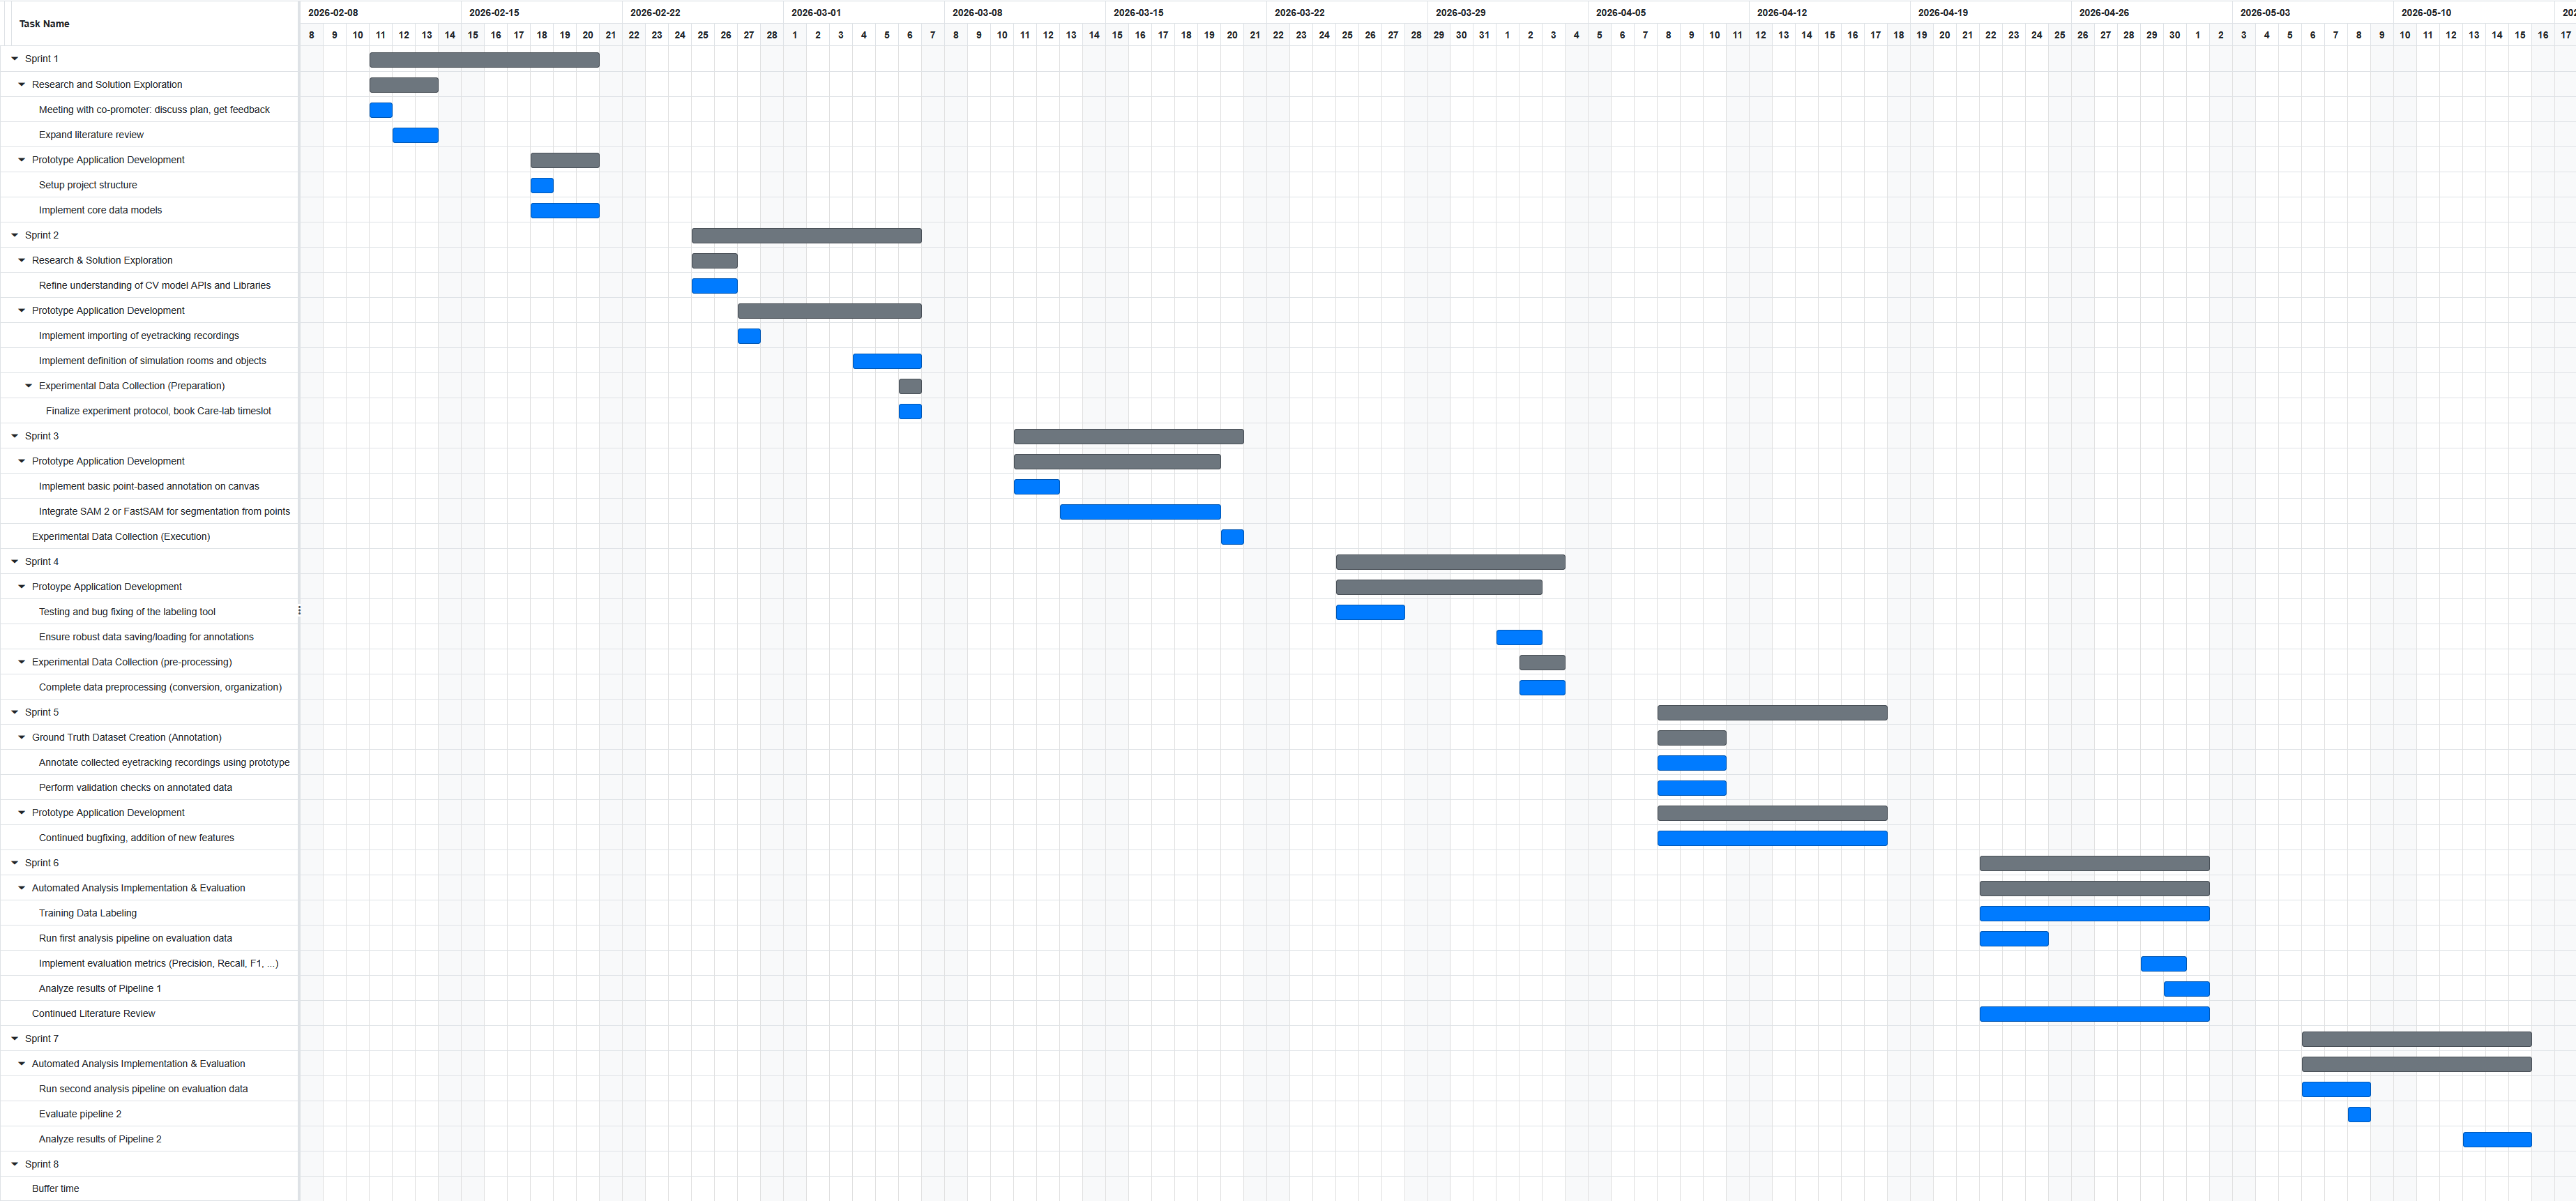
\includegraphics[width=\textwidth]{gantt.png}
  \caption{\label{fig:gantt}Gantt diagram of the research phases and milestones for each sprint.}
\end{figure*}

\section{Expected Results}
\label{sec:expected-results}

Based on the proposed methodology and the current state-of-the-art in computer vision, several outcomes are anticipated from this research.
The primary expectation is the successful development of a functional PoC software application. 
This application will demonstrate the feasibility of integrating computer vision models for automated analysis of observational performance in healthcare simulations.

Regarding the performance of the automated analysis methods, it is hypothesized that object detection models (e.g., fine-tuned YOLO variants or DINO) will yield the most robust and accurate results on the evaluation dataset.
This expectation stems from their inherent design to both localize and classify specific object categories for which they have been trained.
While open-set recognition models like Grounding DINO, or classification approaches based on image embeddings, offer flexibility by not requiring explicit retraining for every new object, they are anticipated to face challenges in this context.\\
The simulated environments contain a multitude of objects, many of which will be \textit{unknown} or irrelevant to the specific set of target objects for a given simulation.
This characteristic of the problem may lead to a higher number of false positives for pure classification models, a known challenge in open-set recognition tasks where the system must distinguish between known classes and a wide array of unseen distractors.
Object detection models, particularly if provided with sufficient training examples of the critical objects, are expected to be more discriminative and less prone to misclassification or false positives.

It is further expected that the system will be able to quantify gaze duration on identified objects with reasonable accuracy.
However, the degree of accuracy is contingent on both the resolution of the eyetracking recordings, and the quality of the provided gaze data.
Thus, it is expected that the system will struggle to accurately detect objects that are far away or not clearly visible in the eyetracking recordings. 

\section{Discussion, Expected\\ Conclusion}
\label{sec:discussion-conclusion}

The primary contribution of this research is expected to be a demonstration of the feasibility of integrating computer vision models with eyetracking data to objectively analyze performance in healthcare simulations.
While the PoC itself will be a prototype and not a production-ready application with comprehensive visualization dashboards, it will provide a solid foundation for future iterations and enhancements.
The instructors at HOGENT's 360° Care-lab will benefit from the clear indication that automated, objective assessment methods are achievable.

As computer vision is a rapidly developing\\ field, it is also anticipated that future advancements, particularly the continued rise of large foundation models, may enable even more sophisticated analysis methods. 
These could potentially allow for the analysis of eyetracking recordings with reduced reliance on extensive, domain-specific training datasets, though current computational costs for such large models can be a limiting factor. 
This research, therefore, not only addresses a current need but also positions the Care-lab to leverage future technological\\ progress in this domain.

\printbibliography[heading=bibintoc]

\end{document}